\section{Auswertung}
\label{sec:Auswertung}
% \subsection{Fehlerrechnung}
% Der Mittelwert einer physikalischen Größe $a$ mit $N$ Einzelmesswerten ist gegeben durch
% \begin{equation}\label{eq:mean}
%     \overline{x}=\frac{1}{N}\sum_{i=1}^Na_\text{i}\,.
% \end{equation}
% Die Standardabweichung eines Mittelwerts zu einer physikalischen Größe a bestimmt sich mit
% \begin{equation}\label{eq:std}
%     \Delta{x}=\sqrt{\frac{1}{N(N-1)}\sum_{i=1}^N\left(a_\text{i}-\overline{x}\right)}\,.
% \end{equation}

% \begin{table}[H]
%   \centering
%   \caption{}
%   \label{tab:}
%   \begin{tabular}{S[table-format=2.1] S[table-format=4] S[table-format=2.1] S[table-format=4]S[table-format=3]S[table-format=2.1]}
%       \toprule
%       {}&{}&{}&{}&{}\\
%       \midrule
      
%       \bottomrule
%   \end{tabular}
% \end{table}

% \begin{figure}[H]
%   \centering
%   \includegraphics{build/}
%   \caption{.}
%   \label{fig:}
% \end{figure}
\subsubsection{Laser Schwelllenstrom (Threshold Current)}
\label{sec:threshold}
Die Stromstärker bei welcher die Diode von LED-Licht auf Laserlicht wechselt wird mit
\begin{equation*}
    I_{\text{th}} = \SI{34.5}{\milli\ampere} \, .
\end{equation*}
In der Abbildung \ref{fig:threshold} ist die das von der Diode emittierte Licht bei einer Stromstärke unterhalb des Schwellenstroms \ref{fig:unterhalb_schwellenstrom}
und bei einer Stromstärke oberhalb des Schwellenstroms \ref{fig:oberhalb_schwellenstrom} zu sehen.
\begin{figure}[H]
    \centering
    \begin{subfigure}{0.45\textwidth}
        \centering
        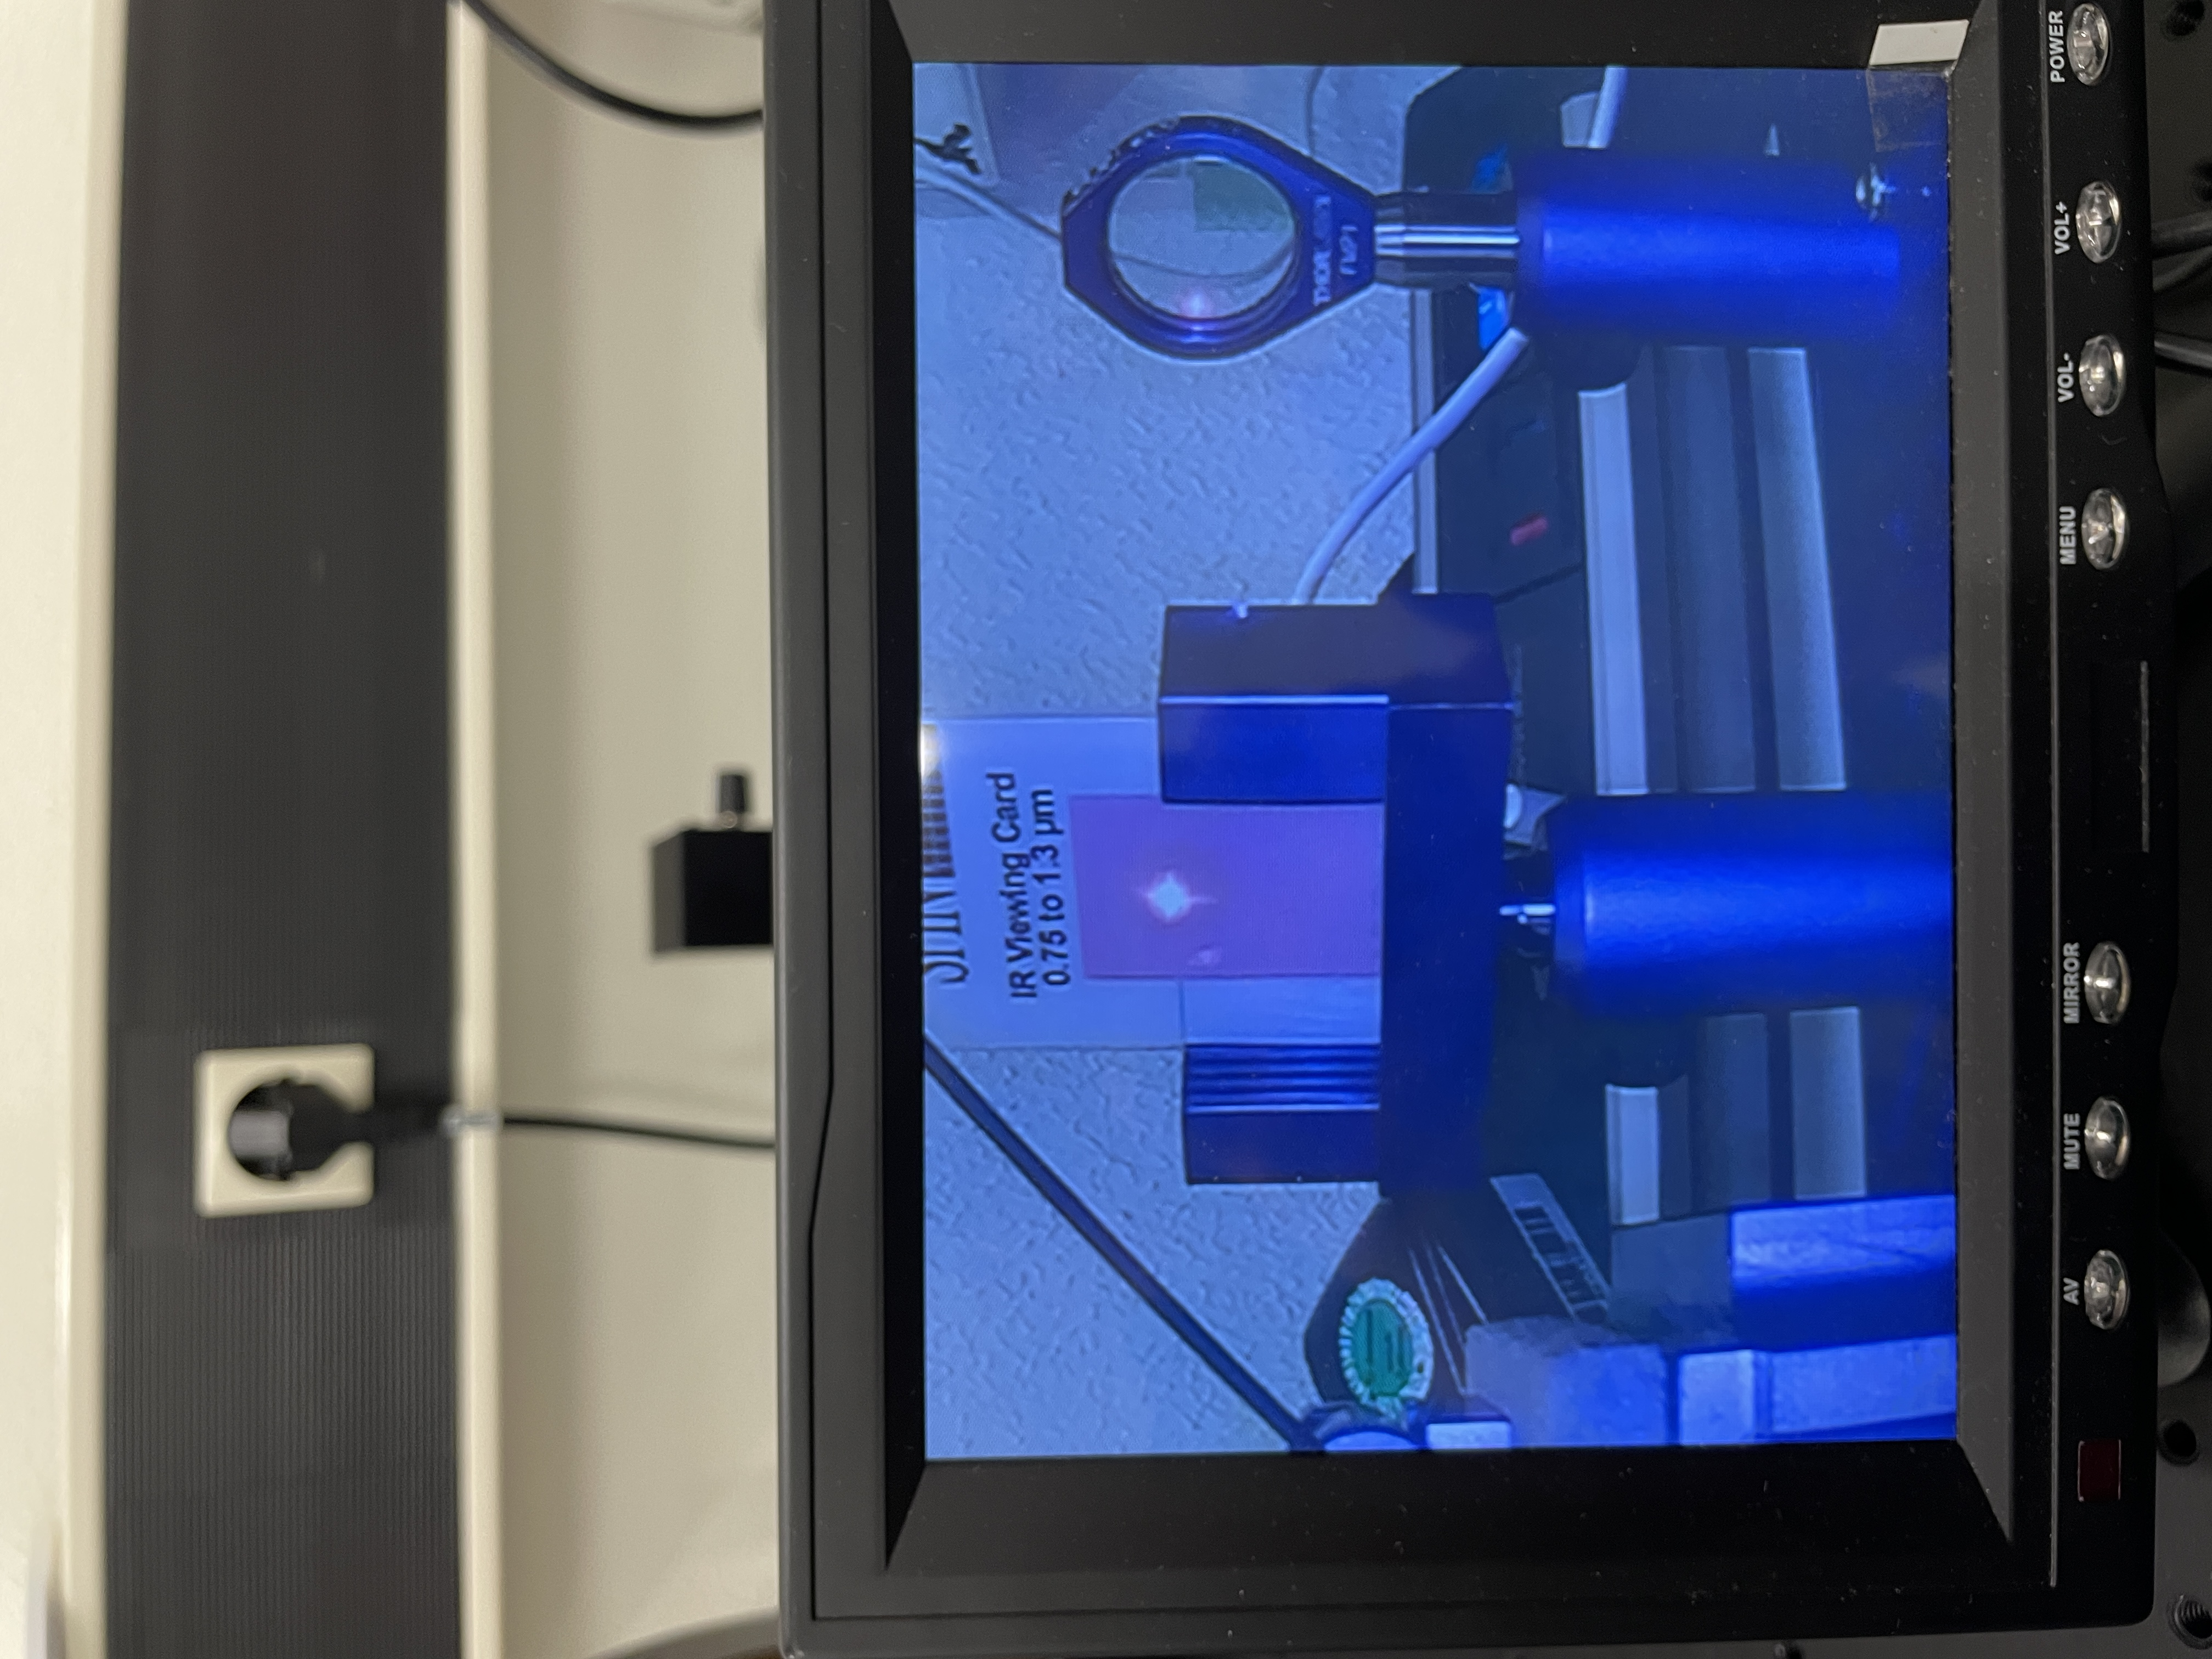
\includegraphics[width=\textwidth]{pictures/LED.JPG}
        \caption{Unterhalb des Schwellenstroms emittiert die Diode LED-Licht.}
        \label{fig:unterhalb_schwellenstrom}
    \end{subfigure}
    \hfill
    \begin{subfigure}{0.45\textwidth}
        \centering
        \includegraphics[width=\textwidth]{pictures/ThresholdLaser.JPG}
        \caption{Oberhalb des Schwellenstroms emittiert die Diode Laserlicht.}
        \label{fig:oberhalb_schwellenstrom}
    \end{subfigure}
    \caption{Vergleich des Diodenbetriebs unterhalb (links) und oberhalb (rechts) des Schwellenstroms.}
    \label{fig:threshold}
\end{figure}

\subsubsection{Rubidium Fluoresszenz}
\label{sec:fluoresszenz}
In der Abbildung \ref{fig:fluoresszenz} ist die Fluoresszenz des Rubidiums zu sehen.
\begin{figure}[H]
    \centering
    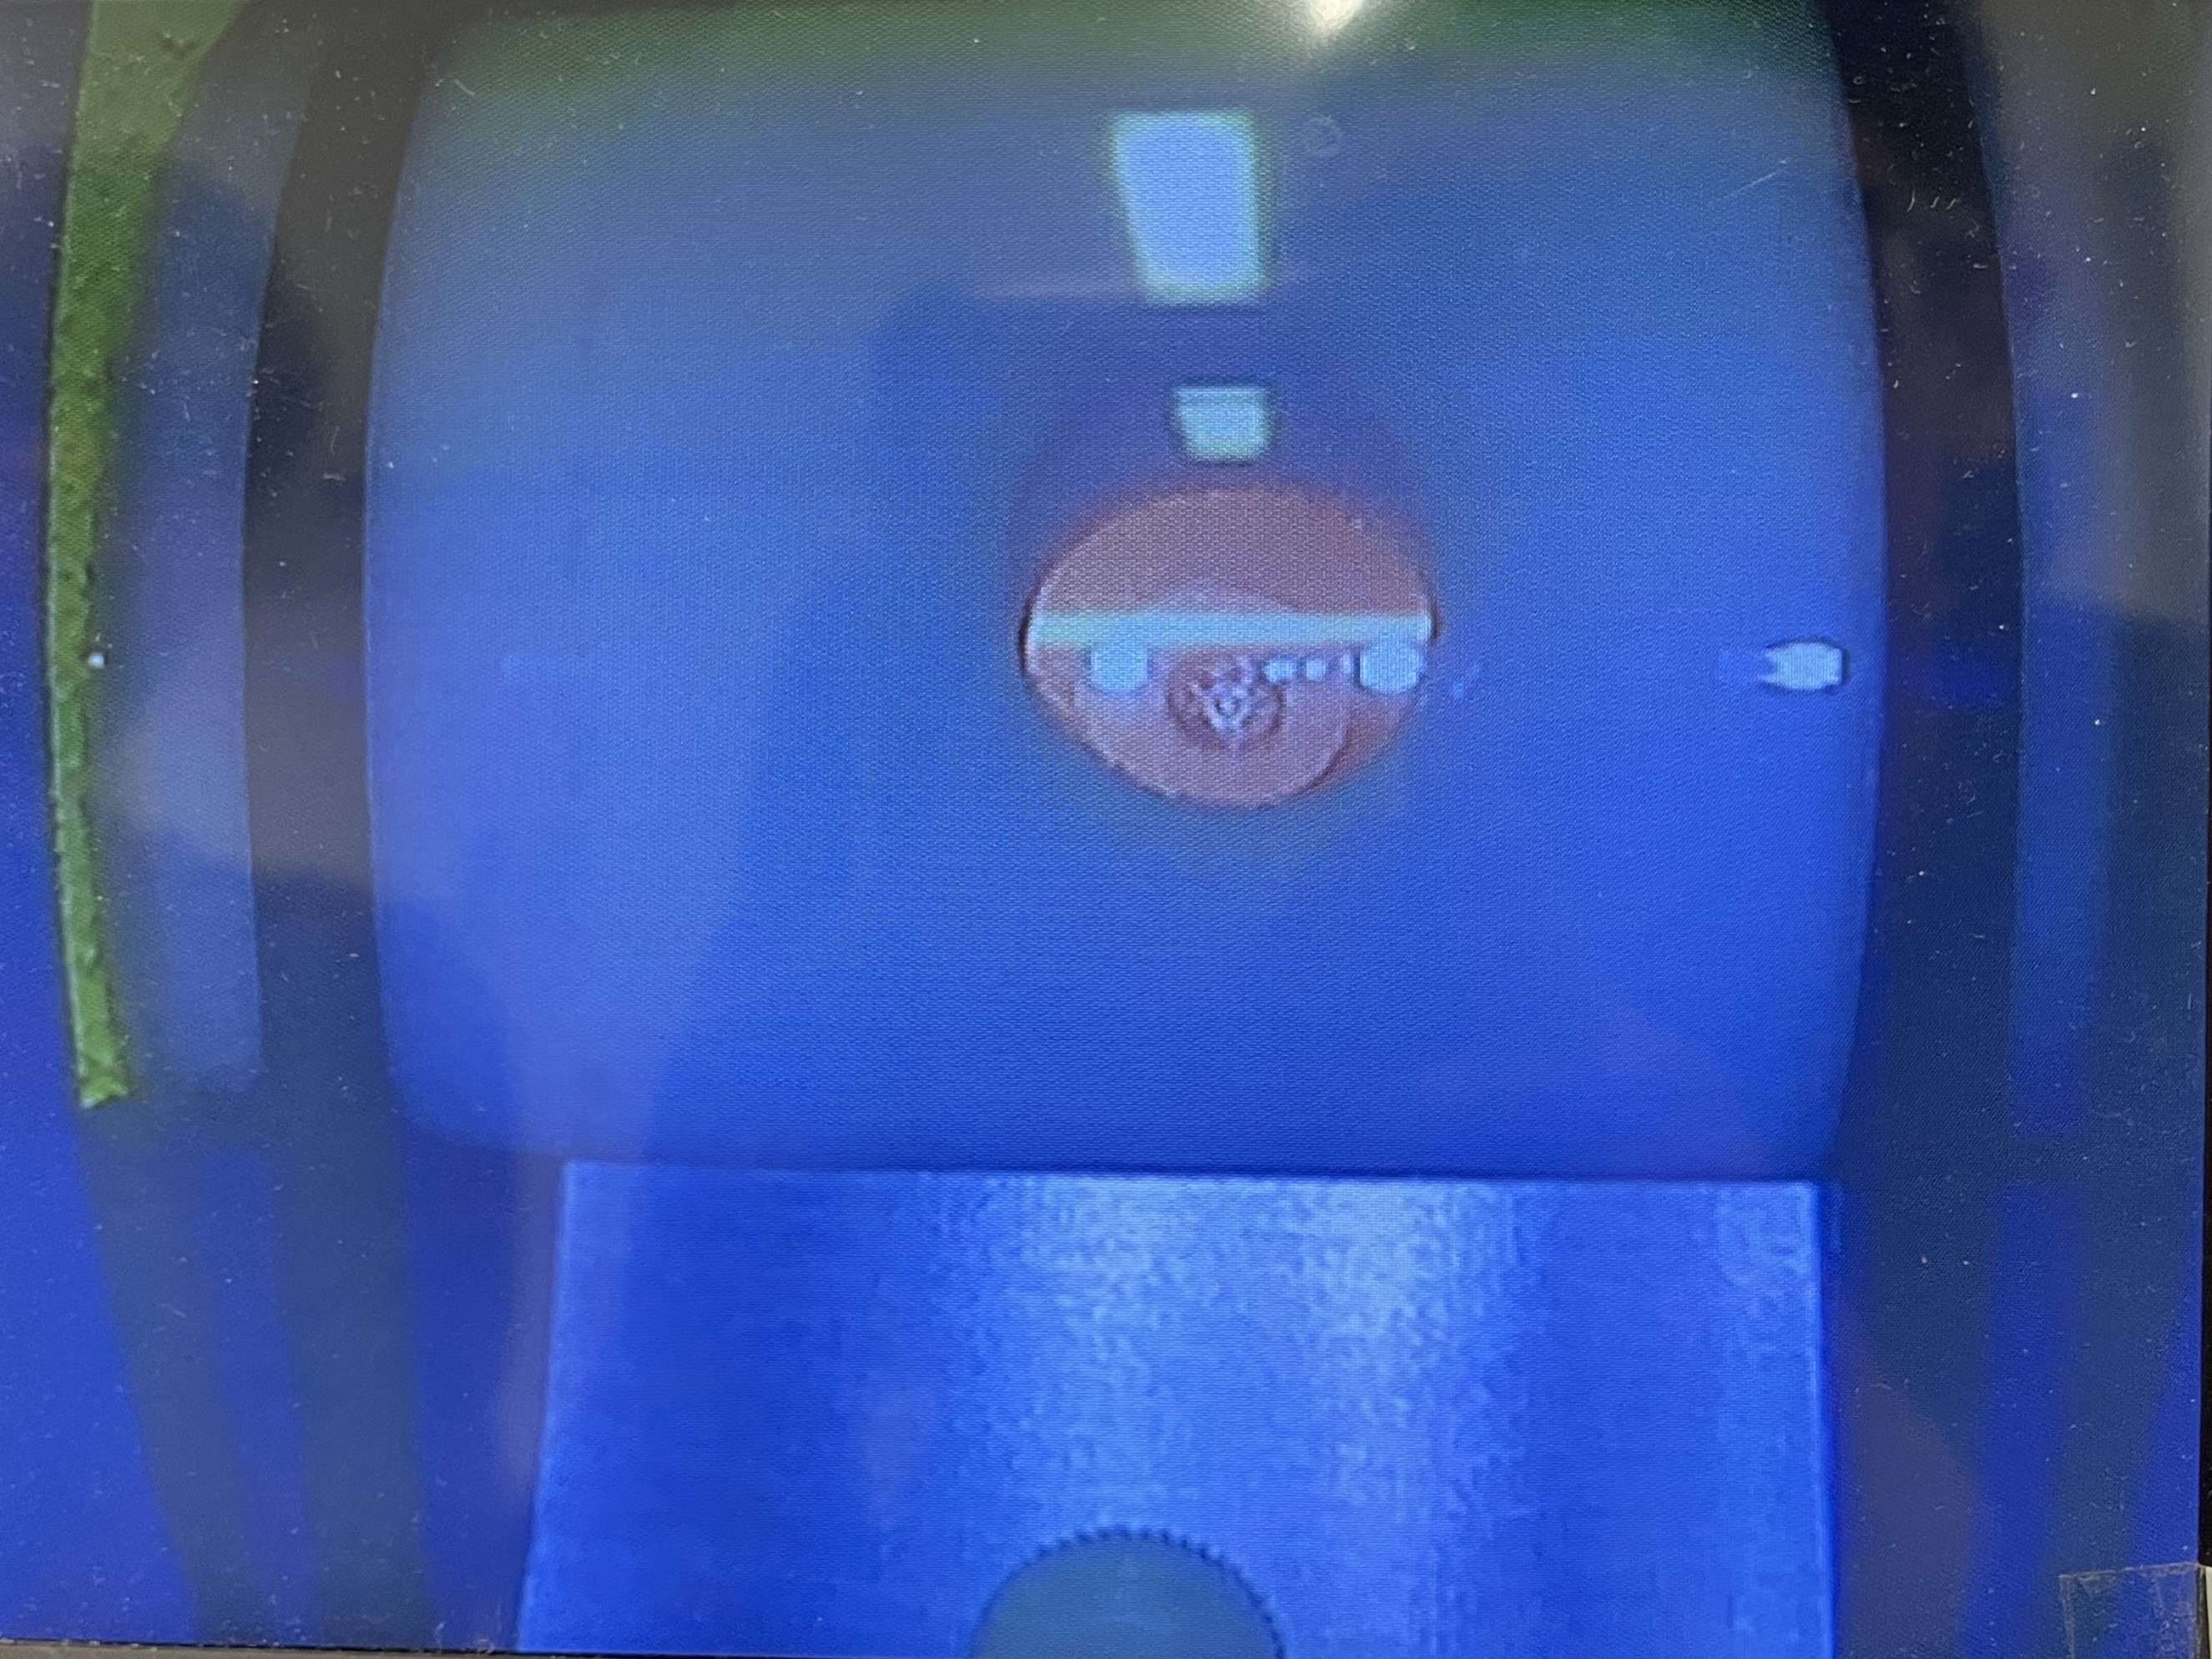
\includegraphics[width=0.5\textwidth]{pictures/Fluoresszenz.JPG}
    \caption{Fluoresszenz des Rubidiums.}
    \label{fig:fluoresszenz}
\end{figure}

\subsubsection{Rubidium Absorptionsspektrum}
\label{sec:absorption}
In der Abbildung \ref{fig:absorption} ist das gemessene Absorptionsspektrum (\ref{fig:absorption_gemessen}) des Rubidiums und die theoretische Erwartung (\ref{fig:absorption_theoretisch}) zu sehen.
\begin{figure}[H]
    \centering
    \begin{subfigure}{0.45\textwidth}
        \centering
        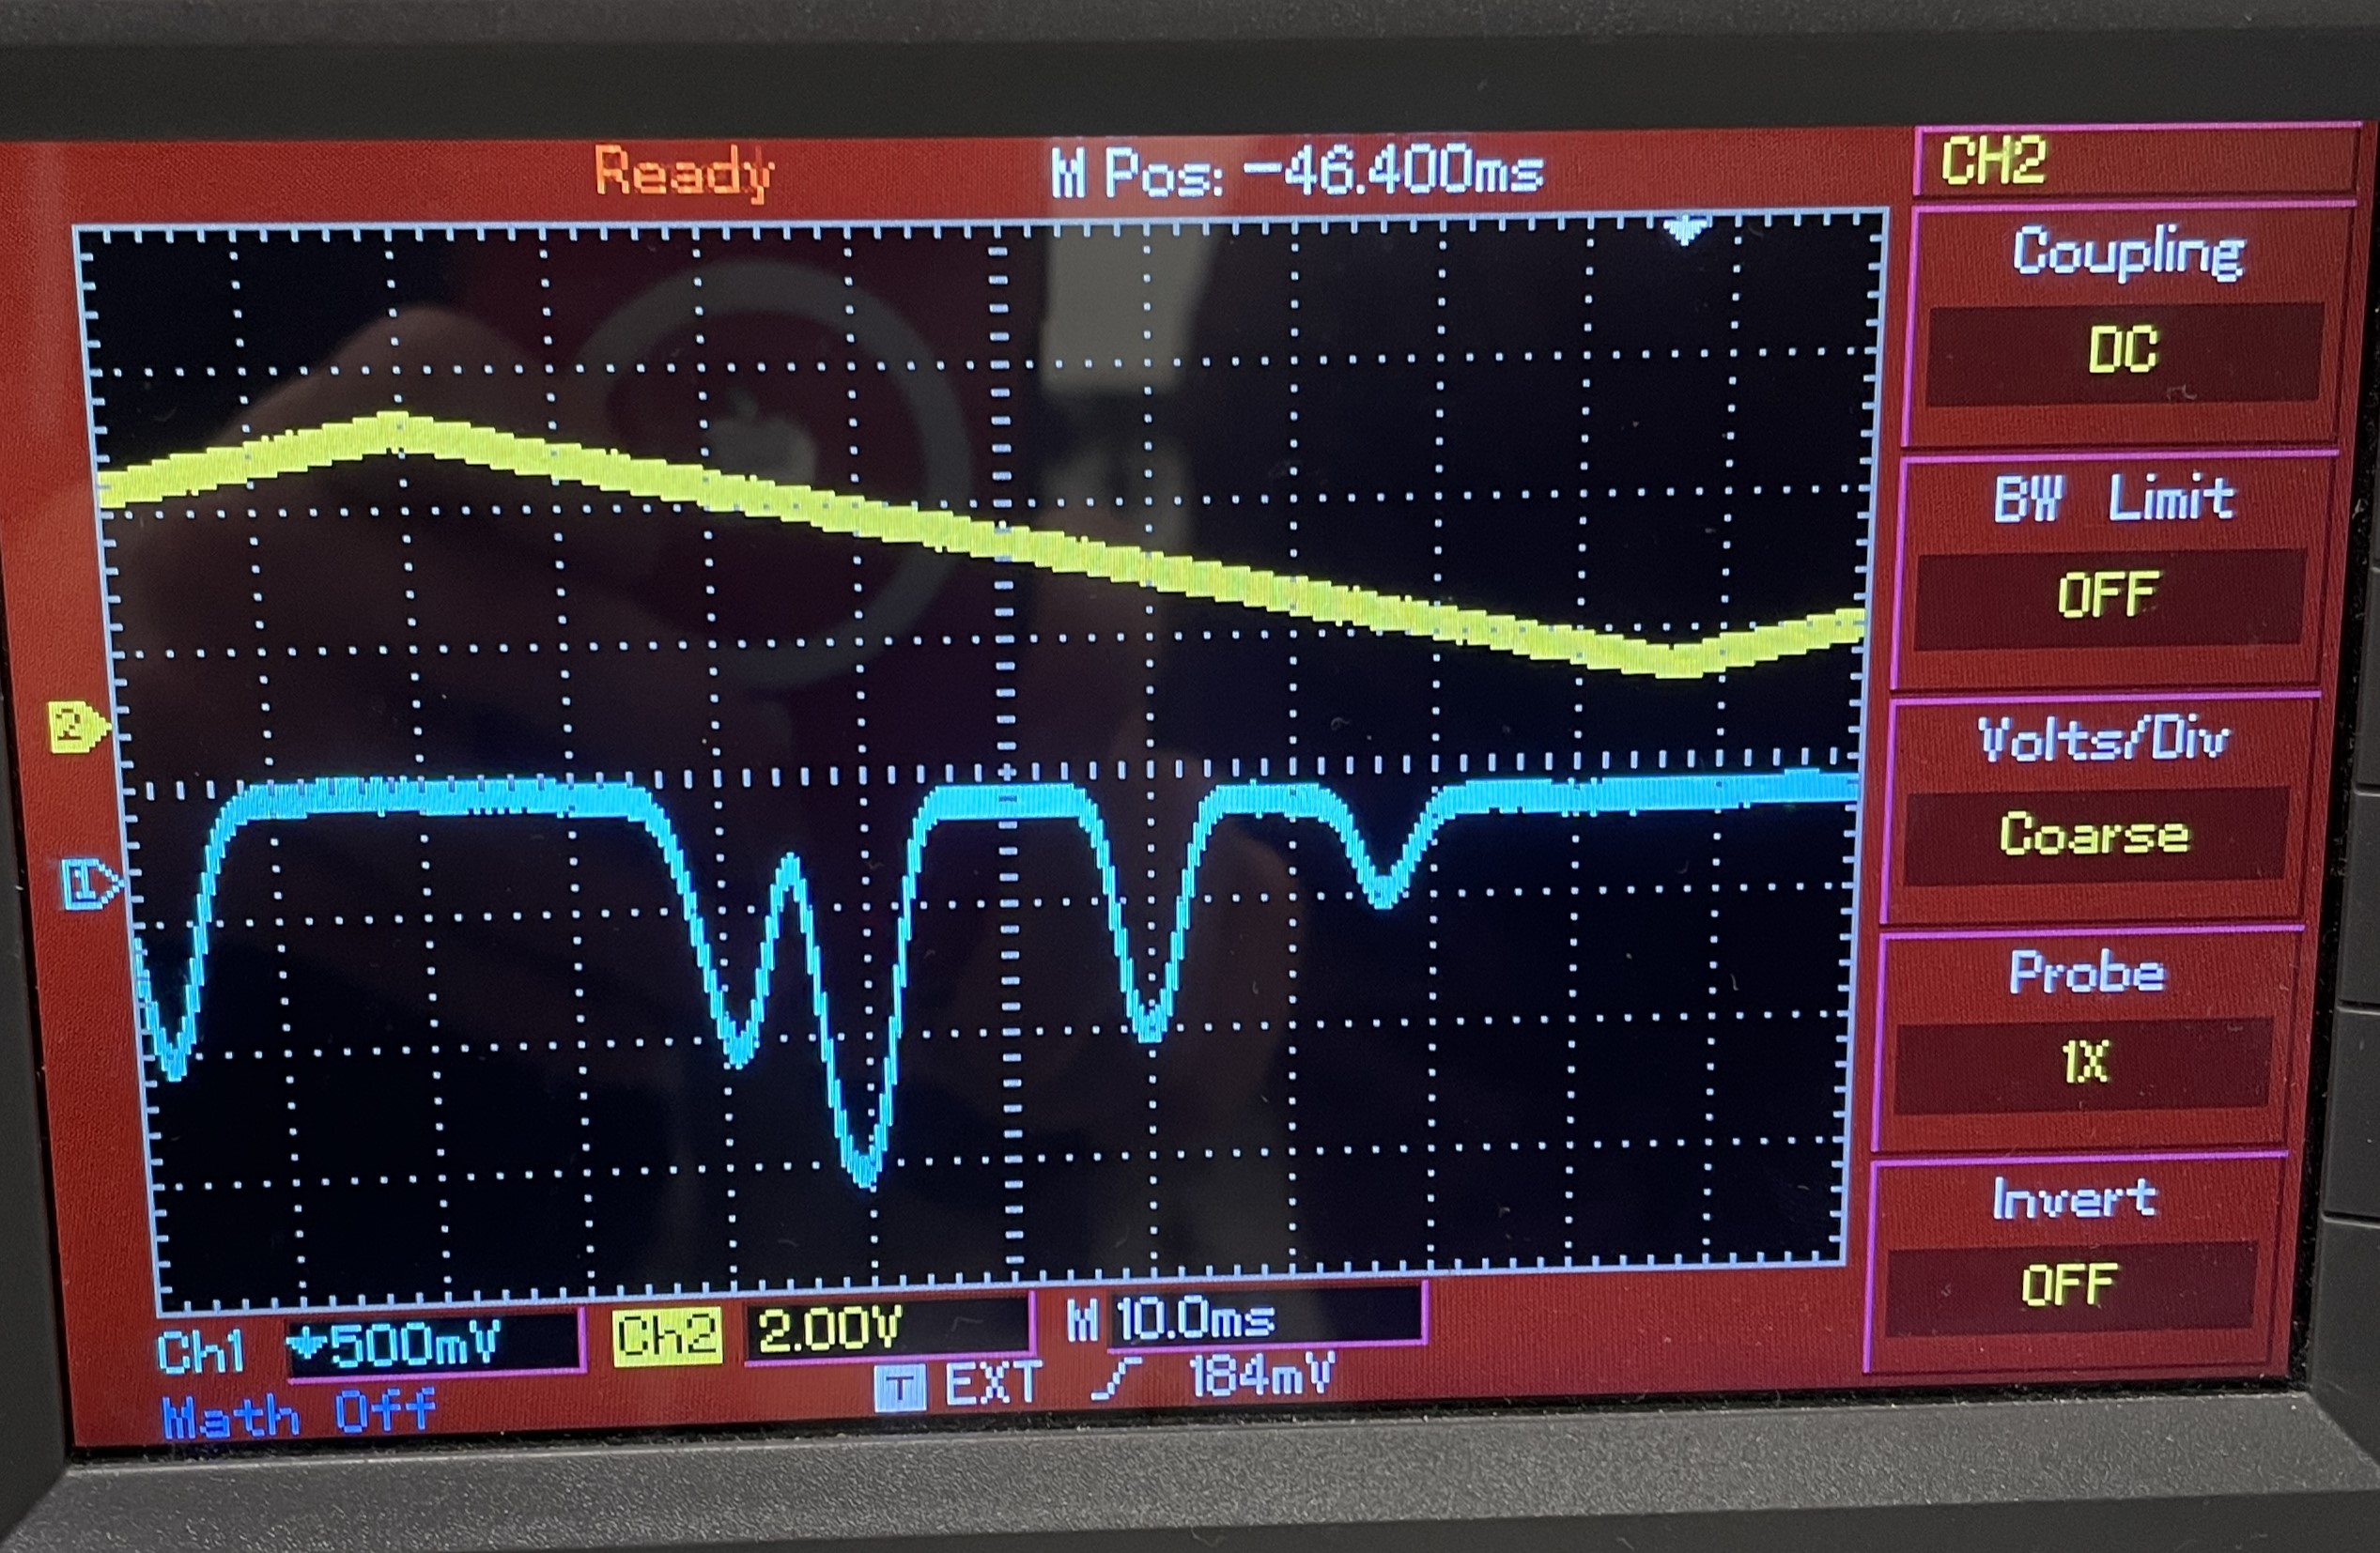
\includegraphics[width=\textwidth]{pictures/AbsorptionsSpektrum.JPG}
        \caption{Gemessenes Absorptionsspektrum des Rubidiums (blau) und die Dreiecksspannung des Generators (gelb) als Funktion der Zeit.}
        \label{fig:absorption_gemessen}
    \end{subfigure}
    \hfill
    \begin{subfigure}{0.45\textwidth}
        \centering
        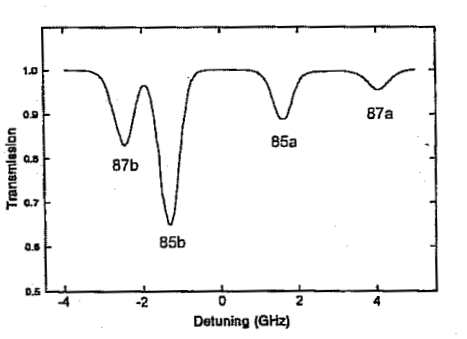
\includegraphics[width=\textwidth]{pictures/absorption_theo.png}
        \caption{Theoretische Erwartung des Absorptionsspektrum von $^{85}$Rb und $^{87}$Rb \cite{teachspin}.}
        \label{fig:absorption_theoretisch}
    \end{subfigure}
    \caption{Gemessenes Absorptionsspektrum des Rubidiums und theoretische Erwartung.}
    \label{fig:absorption}
\end{figure}